\section{Characters and a spin-resolved physical spectrum}
\label{sec:physics-spectrum}

The chiral algebra fixes considerably more physical data than the twelve
lowest conformal weights.  In this section $c_L=c_R=8$, so the quantity
often denoted simply by $c$ in two-dimensional bootstrap plots is $8$;
the sum of the two central charges is $16$.  We distinguish two local
full CFTs throughout:
\begin{equation}\label{eq:physics-two-partitions}
 Z_{\mathrm{diag}}(\tau,\bar\tau)
   =\sum_{i=0}^{11}\chi_i(\tau)\overline{\chi_i(\tau)},
 \qquad
 Z_{E_8}(\tau,\bar\tau)
   =\left|\frac{E_4(\tau)}{\eta(\tau)^8}\right|^2.
\end{equation}
The first uses the diagonal modular invariant of $U$.  The second is
the full theory of the selected holomorphic extension carrying the
Haagerup action constructed later in the manuscript.  They have the
same central charge and different spectra.  In particular a spectral
statement about the diagonal theory must not be assigned to the
holomorphic extension.

\subsection{An exact recurrence and its normalization}

Set $q=e^{2\pi i\tau}$ and write
\[
 \chi_i(q)=q^{h_i-1/3}A_i(q),\qquad
 A_i(q)=\sum_{n\geq0}a_i(n)q^n.
\]
The grading variable $n$ measures distance above the actual lowest
weight, including for $d_3$, whose lowest weight is $15/13$ rather
than its twist representative $2/13$.  The parameter-zero solution of
Evans--Gannon \cite[Sections~1.4 and~2.4]{EG} has the following initial
coefficients; the two rows $a,c_0$ represent distinct simple modules
with equal unflavoured characters.
\begin{center}
\begin{tabular}{c|c|rrrr}
 $i$&$h_i$&$a_i(0)$&$a_i(1)$&$a_i(2)$&$a_i(3)$\\\hline
 $0$&$0$&1&6&120&956\\
 $b$&$1$&80&1250&10630&65042\\
 $a$&$1$&81&1377&11583&71037\\
 $c_0$&$1$&81&1377&11583&71037\\
 $c_1$&$1/3$&3&243&2916&21870\\
 $c_2$&$2/3$&27&594&5967&39852\\
 $d_1$&$6/13$&7&292&3204&23010\\
 $d_2$&$11/13$&42&777&7147&45367\\
 $d_3$&$15/13$&119&1623&12996&76429\\
 $d_4$&$5/13$&5&229&2738&19942\\
 $d_5$&$7/13$&13&347&3804&26390\\
 $d_6$&$8/13$&14&441&4445&30329
\end{tabular}
\end{center}

Here is an explicit recurrence that extends this table without a
lattice-state calculation.  Write
\[
 \Xi=q^\Lambda\sum_{n\geq-1}X_nq^n,
 \quad X_{-1}=I,\quad X_0=\chi,
 \quad C=\chi+[\Lambda,\chi],
\]
where $\Lambda,\chi$ are the rational exponent matrix and integral
characteristic matrix printed in \cite[Section~2.4]{EG}.  They are
also recorded in full in the machine-readable dataset.  With
$J=q^{-1}+196884q+\cdots$, define
\[
 g=\frac{\eta^{24}}{E_4E_6}=\sum_{r\geq0}g_rq^r,
 \qquad
 f=(J-240)g
   =\frac{E_4^2}{E_6}-984g=\sum_{r\geq0}f_rq^r.
\]
Thus $f_0=1$, $f_1=0$, and $g_0=0,g_1=1,g_2=240$.
The differential equation $q\,d\Xi/dq=\Xi(f(\Lambda-I)+gC)$ gives
\begin{equation}\label{eq:physics-xi-recurrence}
 (n+1+\lambda_i-\lambda_j)(X_n)_{ij}
 =\sum_{r=1}^{n+1}
 \left[f_r(\lambda_j-1)(X_{n-r})_{ij}
       +g_r(X_{n-r}C)_{ij}\right].
\end{equation}
All denominators are nonzero.  In particular this specifies the
convolution index directly, independently of typographical renderings
of the $g$ index in equation~(1.24) of the cited paper.  The desired
characters are column zero.  Vacuum grade $n$ uses $(X_{n-1})_{00}$,
whereas nonvacuum grade $n$ uses $(X_n)_{i0}$.

The exporter uses rational arithmetic, caches $X_nC$ once per grade,
and compares the first four printed coefficient columns with the
published data.  An independent oscillator-product calculation checks
\begin{equation}\label{eq:physics-e8-character-identity}
 \frac{E_4}{\eta^8}
 =\chi_0+\chi_b+2\chi_a
 =\chi_0+\chi_b+2\chi_{c_0}
 =q^{-1/3}(1+248q+4124q^2+34752q^3+\cdots)
\end{equation}
through every exported grade.  Equal scalar characters do not choose
between possible extension algebra structures.

\subsection{Removing Virasoro descendants}

We count individual primary components, including their internal
multiplicities, rather than only the twelve extended-algebra sectors.
Let $P(q)=\prod_{m\geq1}(1-q^m)$, and let $v_i(n)$ count Virasoro
highest vectors of weight $h_i+n$ in the $i$th chiral module.  Include
the identity once by setting $v_0(0)=1$.  Then
\begin{equation}\label{eq:physics-primary-extraction}
 \sum_{n\geq0}v_i(n)q^n=P(q)A_i(q)\quad(i\ne0),
 \qquad
 \sum_{n\geq0}v_0(n)q^n=P(q)A_0(q)+q.
\end{equation}
The correction $+q$ removes the nonexistent vacuum state
$L_{-1}\mathbf1$ from the descendant subtraction.

For completeness, the relevant absence of further null vectors can
be seen directly from the Kac determinant
\cite[Lemmas~2--3]{LanglandsVir}.  Parametrize
$c=13-6(t+t^{-1})$; at $c=8$, one has $|t|=1$,
$t+t^{-1}=5/6$, and $\operatorname{Im}t\ne0$.  Its possible singular
weights are
\[
 h_{r,s}=\tfrac14\bigl((r^2-1)t+(s^2-1)t^{-1}-2rs+2\bigr).
\]
For positive integers $r,s$, reality forces $r=s$, in which case
$h_{r,r}=-7(r^2-1)/24\leq0$.  A positive real highest weight therefore
has an irreducible Verma module.  At weight zero the only primitive
null is $L_{-1}\mathbf1$.  Unitarity permits orthogonal removal of
the descendant submodules at each finite grade, giving
\eqref{eq:physics-primary-extraction}.  For example,
\[
 (v_0(0),v_0(1),v_0(2),v_0(3),v_0(4))
 =(1,6,113,830,4934).
\]
The corresponding first nonvacuum grades are
\begin{center}
\begin{tabular}{c|rrrr@{\qquad}c|rrrr}
 $i$&$v_i(0)$&$v_i(1)$&$v_i(2)$&$v_i(3)$&
 $i$&$v_i(0)$&$v_i(1)$&$v_i(2)$&$v_i(3)$\\\hline
 $b$&80&1170&9300&53162&$d_1$&7&285&2905&19514\\
 $a,c_0$&81&1296&10125&58077&$d_2$&42&735&6328&37443\\
 $c_1$&3&240&2670&18711&$d_3$&119&1504&11254&61810\\
 $c_2$&27&567&5346&33291&$d_4$&5&224&2504&16975\\
 &&&&&$d_5$&13&334&3444&22239\\
 &&&&&$d_6$&14&427&3990&25443
\end{tabular}
\end{center}
Every exported chiral character is reconstructed independently by
convolving these multiplicities with the partition numbers and using
the vacuum correction.  This verifies descendant subtraction through
the stated grade; it is not a separate existence proof for $U$.

\subsection{The diagonal theory: scalars and spinning operators}

An ordered pair of grades $(n,m)$ in sector $i$ has
\begin{equation}\label{eq:physics-spectrum-formula}
\begin{gathered}
 (h,\bar h)=(h_i+n,h_i+m),\quad
 \Delta=2h_i+n+m,\quad s=n-m,\\
 d_{\rm states}=a_i(n)a_i(m),\quad
 d_{\rm prim}=v_i(n)v_i(m).
\end{gathered}
\end{equation}
The last quantity counts primaries under both Virasoro algebras.
It includes chiral currents paired with the right vacuum, and vice
versa.  Summing equal $(\Delta,s)$ entries produces the spin-resolved
tables in the dataset.  Character grades through $N$ suffice for the
complete spectrum through $\Delta=N$, because all lowest weights
are nonnegative.  Rectangular products at larger $\Delta$ would
generally be incomplete and are not reported as complete levels.

The seven relevant scalar levels are
\begin{equation}\label{eq:physics-relevant-scalars}
\begin{array}{c|rrrrrrr}
 \Delta&2/3&10/13&12/13&14/13&16/13&4/3&22/13\\\hline
 d_{\rm prim}&9&25&49&169&196&729&1764
\end{array}
\end{equation}
and contain $2941$ primary components in total.  These are the squares
of the seven relevant chiral ground-space dimensions.  No scalar
descendant can enter below dimension two: equality of left and right
weights requires $n=m$, so a positive grade raises $\Delta$ by at
least two.

\IfFileExists{c8_physics_20260927/figures/physics_primary_spectrum.pdf}{%
\begin{figure}[htbp]
\centering
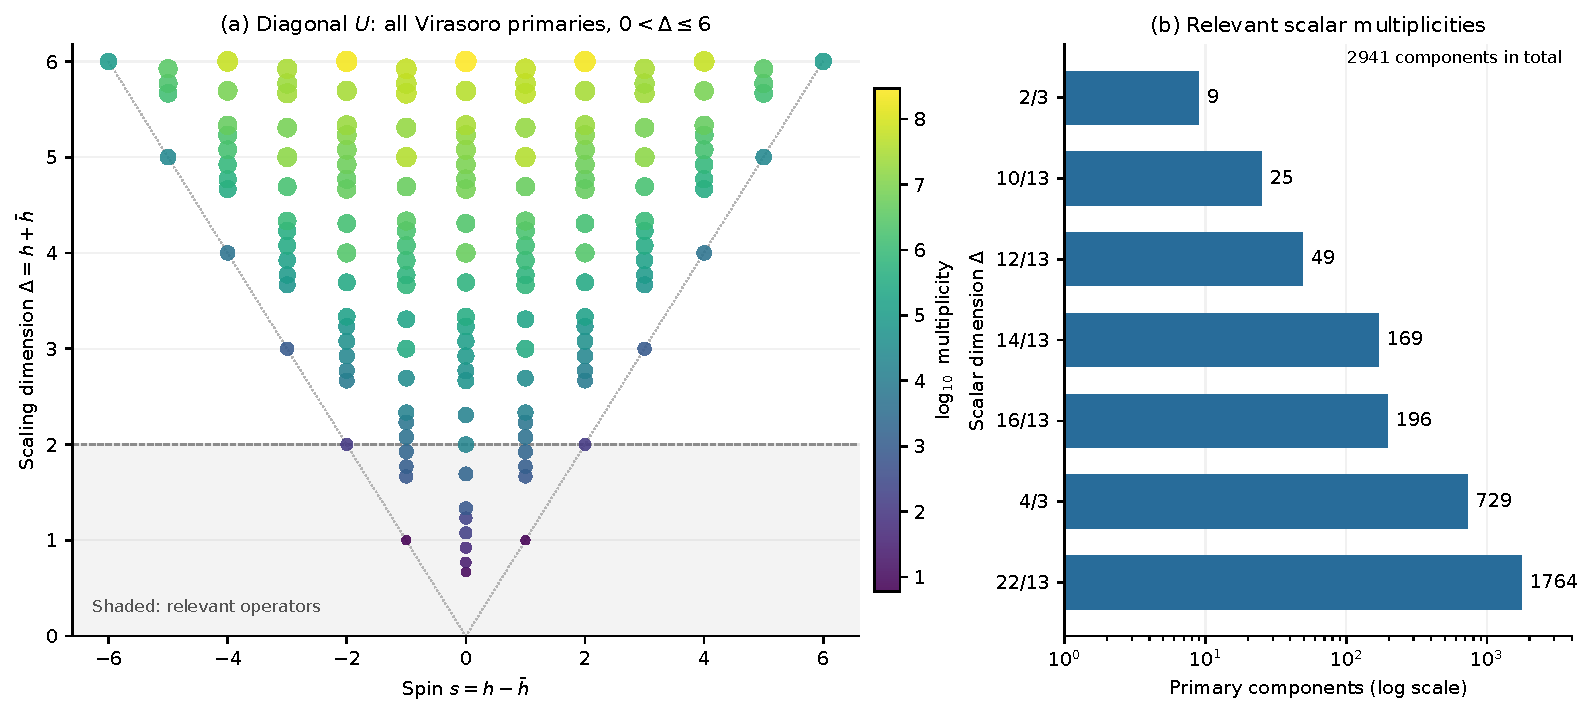
\includegraphics[width=\linewidth]{c8_physics_20260927/figures/physics_primary_spectrum.pdf}
\caption{Exact Virasoro-primary spectrum of the diagonal $U$ theory.
Left: all nonidentity $(\Delta,s)$ levels with $0<\Delta\leq6$,
aggregated over the twelve extended sectors; color and marker area
increase with the logarithm of the component multiplicity. The shaded
region has $\Delta<2$. Right: all seven relevant scalar levels,
with their exact multiplicities and a logarithmic count axis.
The identity and Virasoro descendants are excluded.}
\label{fig:physics-primary-spectrum}
\end{figure}
}{}

The complete additional relevant primary levels with nonzero spin
are
\[
\begin{array}{c|c|r}
 \Delta&s&\text{multiplicity for each displayed spin}\\\hline
 1&\pm1&6\\
 5/3&\pm1&720\\
 23/13&\pm1&1120\\
 25/13&\pm1&1995
\end{array}
\]
For example, the second line is $3(243-3)=720$: the three
$c_1$ ground states pair with its $240$ new grade-one Virasoro
primaries.  Including scalars, there are $10623$ nonidentity relevant
Virasoro-primary components.  The ordinary primary gap and the scalar
primary gap are both $2/3$.  There are six currents in each chirality,
generating the affine subalgebra
$\mathfrak{sl}_{2,1}\oplus\mathfrak{sl}_{2,39}$.

At dimension two the scalar-primary multiplicity is
\begin{equation}\label{eq:physics-diagonal-marginal-count}
 80^2+81^2+81^2+6^2=19558.
\end{equation}
The first three terms are the ground spaces of $b,a,c_0$; the final
term comprises the current bilinears $J^A\bar J^B$.  In addition there
are $113$ chiral weight-two primaries in each spin $\pm2$ channel.
Thus dimension two contains $19784$ Virasoro-primary components and
$19798$ states.  The difference consists of the two stress tensors
and twelve current derivatives.  We call dimension-two scalars
\emph{marginal by dimension}; their beta functions and exact
marginality require OPE data not fixed by the character vector.

\subsection{The holomorphic extension and symmetry-preserving perturbations}

For the full $E_8$ theory, the same descendant subtraction gives
$248$ chiral weight-one and $3875$ chiral weight-two Virasoro
primaries.  Consequently its ordinary primary gap is one, its scalar
primary gap is two, and it has no relevant scalar.  The
$\Delta=2$ scalar space has dimension $248^2=61504$; the total
dimension-two state multiplicity is
$2\cdot4124+248^2=69752$.

For the selected canonical extension, the defect construction below
specifies a first chiral $\mathcal H_3$ action inside the full
$\mathcal H_3\boxtimes\mathcal H_3^{\mathrm{op}}$ defect category.
Its invariant Hilbert space is
$U\otimes\overline{H'}$: the first factor acts in its vacuum
representation on $U$ and leaves the antiholomorphic extension
unrestricted.  It therefore has exactly $6\cdot248=1488$ invariant
scalar components at dimension two.  Requiring invariance under
\emph{both independent factors} instead gives
$U\otimes\overline U$ and $6^2=36$ such components.  Each convention
has invariant scalar gap exactly two.  These invariant counts use
the specified canonical-extension defect action, not only the
unflavoured character identity.  Neither count establishes an exactly
marginal family: that requires the corresponding OPE coefficients
and beta functions.

\subsection{Finite-temperature observables with controlled tails}

On a circle of circumference $L$ and velocity $v$, set
$t=\beta v/L$, $b=2\pi t$ and $E=\Delta-2/3$.  Then
\[
 H=\frac{2\pi v}{L}E,\qquad
 P=\frac{2\pi}{L}s,\qquad
 Z(b)=\sum_{\Delta,s}d_{\Delta,s}e^{-b(\Delta-2/3)}.
\]
The ground energy is $-4\pi v/(3L)$.  The exact finite spectral table
already gives a lower bound on $Z$ at every positive temperature.
The following elementary modular estimate also controls the omitted
tail and makes a finite-temperature table quantitatively meaningful.

\begin{proposition}[A tail bound from modular invariance]
\label{prop:physics-modular-tail}
Suppose $Z(b)=Z(4\pi^2/b)$ has nonnegative degeneracies, and that all
states with $\Delta\leq D$ are known, where $D>2/3$.  Write
$Z=L_D+H_D$ for its known and omitted sums, and put
$E_D=D-2/3$.  If $b>2\pi$ and $b'=4\pi^2/b$, then
\begin{equation}\label{eq:physics-thermal-tail}
 0\leq H_D(b)\leq
 \frac{L_D(b)-L_D(b')}{e^{(b-b')E_D}-1}.
\end{equation}
At $b=2\pi$ one has
$0\leq H_D(b)\leq L_D'(b)/E_D$.
For $b<2\pi$ the same bounds apply to $Z(b')=Z(b)$.
\end{proposition}
\begin{proof}
Every omitted energy exceeds $E_D>0$, hence
$H_D(b)\leq rH_D(b')$ with $r=e^{-(b-b')E_D}<1$.
Modular invariance gives
$H_D(b')=H_D(b)+L_D(b)-L_D(b')$; rearranging yields
\eqref{eq:physics-thermal-tail}.  At the fixed point $Z'(2\pi)=0$,
so $L_D'(2\pi)=-H_D'(2\pi)\geq E_DH_D(2\pi)$.
\end{proof}

The real-number rearrangement and the positive-division step at the
fixed point are formalized as
\artifact{modular_heavy_tail_comparison} and
\artifact{selfdual_tail_first_moment_comparison} in
\artifact{lean/HaagerupIzumi/CFT/PhysicsBounds.lean}.
Their hypotheses explicitly include the balance, contraction, and
first-moment inequalities used above. They do not formalize spectral
convergence, the modular functional equation, differentiation of
the trace, or the decimal interval implementation. The guarded
compiler and axiom report is
\artifact{c8_physics_20260927/physics_lean.log}.

To control energy and heat capacity, choose $0<b_0<b$ and bound
$H_D(b_0)$ by the same proposition.  For $k=1,2$,
\begin{equation}\label{eq:physics-moment-tail}
 \sum_{\Delta>D,s}d_{\Delta,s}E^ke^{-bE}
 \leq H_D(b_0)\sup_{E\geq E_D}E^ke^{-(b-b_0)E}.
\end{equation}
The supremum occurs at $E_D$ when $(b-b_0)E_D\geq k$, and otherwise
at $k/(b-b_0)$.  Together with the exact low-energy moments this bounds
$\langle E\rangle$, $C_V=b^2\operatorname{Var}(E)$, and
$S=\log Z+b\langle E\rangle$.  At $t=1$, modular invariance fixes
$\langle E\rangle=0$ exactly.

The supplied thermal tables use $D=24$ and
$t=1/2,3/4,1,3/2,2$, with $b_0=0.9b$ for moment bounds.
The implementation propagates closed decimal intervals with outward
rounding and a rational enclosure of $\pi$; the tables report both
endpoints. The supplied $100$-digit enclosure of $\pi$ is independently
checked by rational alternating sums in Machin's identity
$\pi=16\arctan(1/5)-4\arctan(1/239)$, using $80$ and $25$ terms
with explicit next-term bounds. Their certification is conditional on positivity and
modular invariance of the full CFT, which are mathematical premises
established elsewhere, and not consequences of finite coefficient
agreement.  No unbounded-temperature accuracy claim is made.

For direct comparison the following values are rounded from those
intervals.  Every displayed number has absolute error less than
$10^{-6}$, including both rounding and the omitted-state tail;
the exporter checks this containment before producing the table.
\begin{center}\small
\begin{tabular}{c|c|rrrr}
theory & $t$ & $Z$ & $\langle\Delta-2/3\rangle$ & $C_V$ & $S$\\\hline
$U$ diagonal & $1/2$ & 4367.819471 & 2.653128 & 17.089150 & 16.717068\\
$U$ diagonal & $3/4$ & 303.785760 & 0.983857 & 16.343538 & 10.352640\\
$U$ diagonal & $1$ & 147.219258 & 0.000000 & 19.266968 & 4.991923\\
$U$ diagonal & $3/2$ & 565.179187 & -0.621644 & 3.473060 & 0.478284\\
$U$ diagonal & $2$ & 4367.819471 & -0.663282 & 0.419054 & 0.046971\\
$E_8$ full & $1/2$ & 4356.000000 & 2.659753 & 16.984459 & 16.735170\\
$E_8$ full & $3/4$ & 297.792228 & 0.991916 & 16.622062 & 10.370689\\
$E_8$ full & $1$ & 144.000000 & 0.000000 & 19.157072 & 4.969813\\
$E_8$ full & $3/2$ & 557.169604 & -0.627321 & 3.435582 & 0.410512\\
$E_8$ full & $2$ & 4356.000000 & -0.664938 & 0.272738 & 0.023449\\
\end{tabular}

\end{center}

\IfFileExists{c8_physics_20260927/figures/physics_thermal_comparison.pdf}{%
\begin{figure}[htbp]
\centering
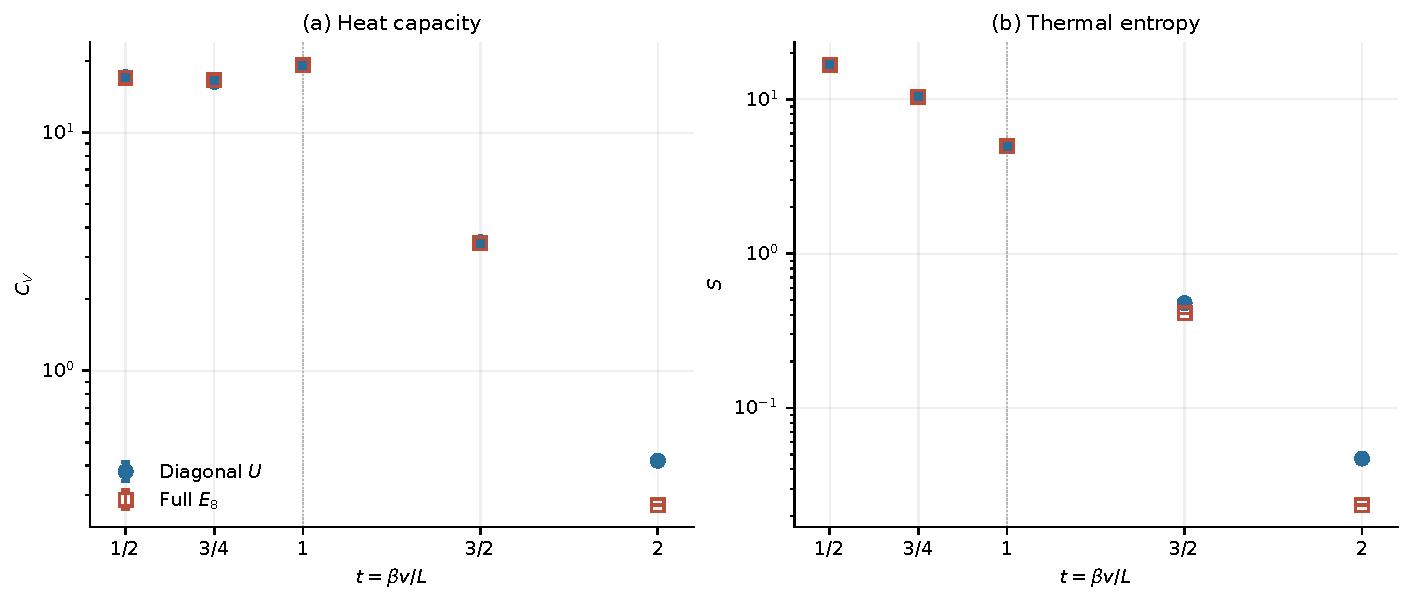
\includegraphics[width=\linewidth]{c8_physics_20260927/figures/physics_thermal_comparison.pdf}
\caption{Heat capacity and thermal entropy of the two full theories at
the five computed temperatures $t=\beta v/L$. Both vertical axes are
logarithmic. No interpolation is drawn. Error bars come from the
conditional certified intervals using all states through $\Delta=24$
and the modular/moment tail bounds; they are smaller than the markers.
The dotted line marks the modular fixed point $t=1$.}
\label{fig:physics-thermal}
\end{figure}
}{}

In the thermodynamic limit both theories have
\[
 f(T)-f(0)=-\frac{4\pi}{3v}T^2,
 \qquad s(T)=\frac{C_V(T)}L=\frac{8\pi}{3v}T.
\]
Their universal single-interval ground-state entanglement coefficient
is $8/3$ in front of $\log(\ell/\epsilon)$, and the R\'enyi coefficient
is $\frac43(1+n^{-1})$.  These central-charge observables do not
distinguish the diagonal theory from its holomorphic extension;
the low-energy spectrum and defect-resolved observables do.

\subsection{Dataset, reproducibility, and limits}

The standalone standard-library producer is
\artifact{c8_physics_20260927/spectrum.py}.  Its default run computes
24 grades of all twelve characters, including Virasoro-primary
multiplicities, and complete spectra through $\Delta=24$ for both
full theories.  The output directory contains
\artifact{characters.json}, \artifact{characters.tsv},
\artifact{fundamental_matrix.json},
\artifact{diagonal_sector_spectrum.tsv},
\artifact{diagonal_spectrum.tsv}, \artifact{e8_spectrum.tsv},
\artifact{scalars.tsv}, \artifact{low_spectrum.json},
\artifact{thermal.json}, and \artifact{thermal.tsv}.
The run summary records coefficient controls, nonnegative integrality,
descendant reconstruction, spin reflection, the $E_8$ product check,
and source/output hashes.  Paths in this paragraph are relative to
\artifact{c8_physics_20260927/data/}, except the explicitly named
producer.

For a replay into a fresh directory, run serially from the repository
root (ordinary Python, without optimization):
\begin{verbatim}
python hi_cft_safe_run.py --limit-mib 512 -- \
  python c8_physics_20260927/spectrum.py --order 24 --delta-cut 24 \
  --outdir /tmp/c8-physics-spectrum-replay
\end{verbatim}
Existing output files are not overwritten. The address cap in this
command is lower than the permanent machine limit; the launcher also
retains its host-memory reserve, process-group watchdog, and two-CPU
limit.

The spectrum exporter determines unflavoured graded dimensions and
the stated thermal observables.  It does not compute normalized
three-point coefficients, crossing matrices of conformal blocks,
defect eigenvectors, or branching characters with Cartan fugacities.
The separate defect and correlator datasets below provide further
information of those kinds in their stated scopes.  In particular an
exclusion plot that resolves Haagerup charges uses the specified
defect-sector decomposition; ordinary unflavoured gaps alone do not
supply its inputs.
